% steps/step04.tex
\section[گام چهارم: طراحی و برچسب‌گذاری داده]{\faPenNib\ \ گام چهارم: طراحی و برچسب‌گذاری داده}
\begin{stepbox}

\field{داده‌ها چگونه ساختاردهی و سازمان‌دهی می‌شوند؟}{
    تصاویر سه‌بعدی \lr{CT Scan} به‌عنوان ورودی سامانه سازمان‌دهی می‌شوند و خروجی‌ها نیز در قالب ماسک‌های سه‌کلاسه استاندارد ساختار می‌یابند: پس‌زمینه با کد ۰، بافت سالم کبد با کد ۱ و تومور با کد ۲. این ساختار یکپارچه، امکان آموزش دقیق و ارزیابی منسجم مدل را فراهم می‌کند.
}

\field{برچسب‌گذاری چگونه انجام می‌شود؟}{
    فرآیند برچسب‌گذاری باید توسط رادیولوژیست‌های مجرب و با استفاده از نرم‌افزارهای تخصصی مانند \lr{ITK-SNAP} به‌صورت دستی و مقطع‌به‌مقطع (\lr{Slice-wise}) روی تصاویر سه‌بعدی انجام شود. این روش، دقت مرزبندی ضایعات و کیفیت \lr{Ground Truth} را به‌طور قابل‌توجهی افزایش می‌دهد.
}

\field{کیفیت و تنوع داده‌ها چگونه تضمین می‌شود؟}{
    برای جلوگیری از بیش‌برازش (\lr{Overfitting}) نسبت به تنظیمات یک دستگاه یا یک مرکز درمانی خاص، داده‌ها به‌صورت چندمرکزی (\lr{Multi-center}) از بیمارستان‌ها و اسکنرهای مختلف جمع‌آوری می‌شوند تا مدل در مواجهه با شرایط متنوع تصویربرداری، تعمیم‌پذیری بالاتری داشته باشد. همچنین برای کاهش خطای انسانی، از یک پروتکل بازبینی چندمرحله‌ای استفاده می‌شود؛ به این صورت که برچسب‌های اولیه توسط یک رادیولوژیست ثبت شده و سپس توسط چند متخصص دیگر به‌صورت مستقل بررسی و تأیید می‌شوند. در صورت وجود اختلاف نظر، تصمیم نهایی بر اساس نظر پزشک ارشد اتخاذ می‌شود.
}


\begin{center}
    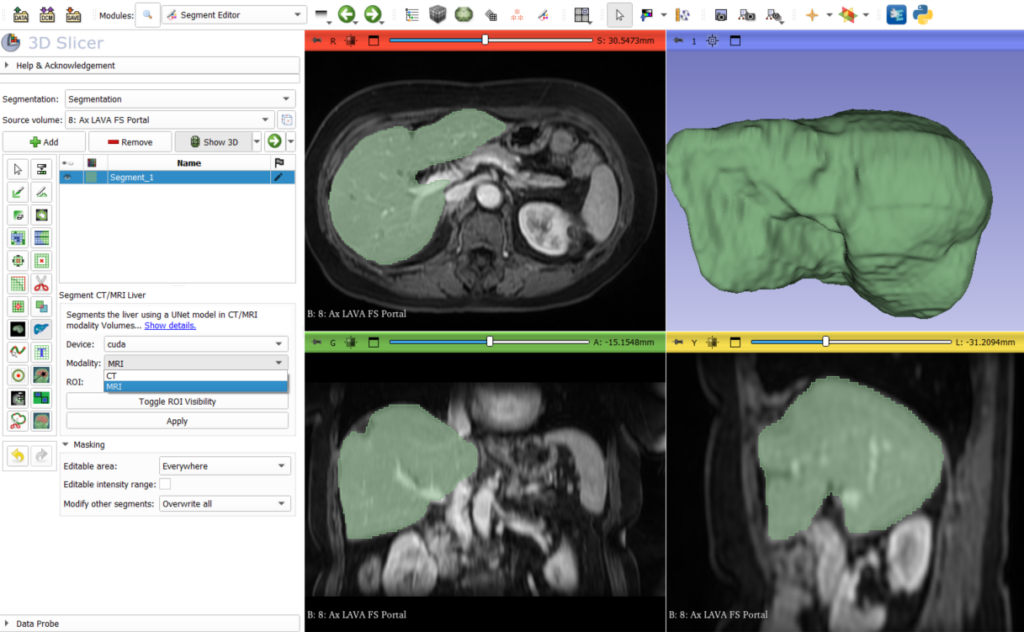
\includegraphics[width=0.85\textwidth]{images/3d-slicer.png}
    \vspace{0.2cm} \\
    \footnotesize{شکل ۴ - محیط نرم‌افزار \lr{3D Slicer} برای نشانه‌گذاری (\lr{Annotation}) و استخراج ماسک کبد در نماهای مختلف سه‌بعدی و دوبعدی}
\end{center}



\end{stepbox}
